% Page Layout
\documentclass[12pt,t]{beamer}
\usepackage{etex} % Avoid an error due to a lack of registers
\usepackage[english]{babel} % Defines the language of macros as well
\usepackage{float}
\usepackage{amsmath}
\usepackage{listings}
\usepackage{geometry}
\usepackage{graphicx}
% Desired Packages
%\usepackage[pdftex]{graphicx}
\usepackage[utf8]{inputenc}
\usepackage{amsmath}
\usepackage{amssymb}
\usepackage{lastpage}
\usepackage{listings}
\usepackage{caption}
\usepackage{xy}
\usepackage{microtype}
\usepackage{lmodern, hfoldsty}
\usepackage{ellipsis}
\usepackage{tabularx}
\usepackage{beamerthemeshadow}
\usepackage{nameref}
\usepackage{hyperref}
\usepackage{subfig}
\usepackage[absolute,overlay]{textpos}
\setlength{\TPHorizModule}{\paperwidth}
\setlength{\TPHorizModule}{\paperheight}

% Further Configurations
\newcommand{\Fat}[1]{{\large \bf \textcolor{cdc_Blue}{#1}}}
\renewcommand\rmdefault{pmy}            		% Activate Myriad Font
\definecolor{Gray}{rgb}{0.5, 0.5, 0.5}  		% Define light color
\definecolor{HighlightRed}{rgb}{0.6, 0.0, 0.0}  % Define light highlighting color
\graphicspath{{images/}}
\usetheme{UniOldbg}                     		% The main thing: our theme


\author{DoWES}
\title{Jan Kämper \& Florian Börgel}
\date{11.10.2016}
\semester{Semester 2016}
\institute{Universität Oldenburg}

\begin{document}

\definecolor{mygreen}{rgb}{0,0.6,0}
\definecolor{mygray}{rgb}{0.5,0.5,0.5}
\definecolor{mymauve}{rgb}{0.58,0,0.82}

\lstset{ %
  backgroundcolor=\color{white},   % choose the background color; you must add \usepackage{color} or \usepackage{xcolor}
  basicstyle=\tiny,        % the size of the fonts that are used for the code
  breakatwhitespace=false,         % sets if automatic breaks should only happen at whitespace
  breaklines=true,                 % sets automatic line breaking
  captionpos=b,                    % sets the caption-position to bottom
  commentstyle=\color{mygreen},    % comment style
  deletekeywords={...},            % if you want to delete keywords from the given language
  escapeinside={\%*}{*)},          % if you want to add LaTeX within your code
  extendedchars=true,              % lets you use non-ASCII characters; for 8-bits encodings only, does not work with UTF-8
  frame=tb,	                   % adds a frame around the code
  keepspaces=true,                 % keeps spaces in text, useful for keeping indentation of code (possibly needs columns=flexible)
  keywordstyle=\color{blue},       % keyword style
  language=Octave,                 % the language of the code
  otherkeywords={*,...},           % if you want to add more keywords to the set
  numbers=left,                    % where to put the line-numbers; possible values are (none, left, right)
  numbersep=5pt,                   % how far the line-numbers are from the code
  numberstyle=\tiny\color{mygray}, % the style that is used for the line-numbers
  rulecolor=\color{black},         % if not set, the frame-color may be changed on line-breaks within not-black text (e.g. comments (green here))
  showspaces=false,                % show spaces everywhere adding particular underscores; it overrides 'showstringspaces'
  showstringspaces=false,          % underline spaces within strings only
  showtabs=false,                  % show tabs within strings adding particular underscores
  stepnumber=2,                    % the step between two line-numbers. If it's 1, each line will be numbered
  stringstyle=\color{mymauve},     % string literal style
  tabsize=2,	                   % sets default tabsize to 2 spaces
  title=\lstname                   % show the filename of files included with \lstinputlisting; also try caption instead of title
}


\frame{\titlepage}
\frame{\frametitle{Table of Contents}\tableofcontents}

\AtBeginSection[]{
	\frame{
		\frametitle{Table of Contents}
		\tableofcontents[currentsection]
	}
}

%%%%%%%%%%%% Start of content %%%%%%%%%%%% 
\section{Selection of Main Parameters}

\begin{frame}
\huge 
Formulas
\begin{figure}[htbp]
\centering
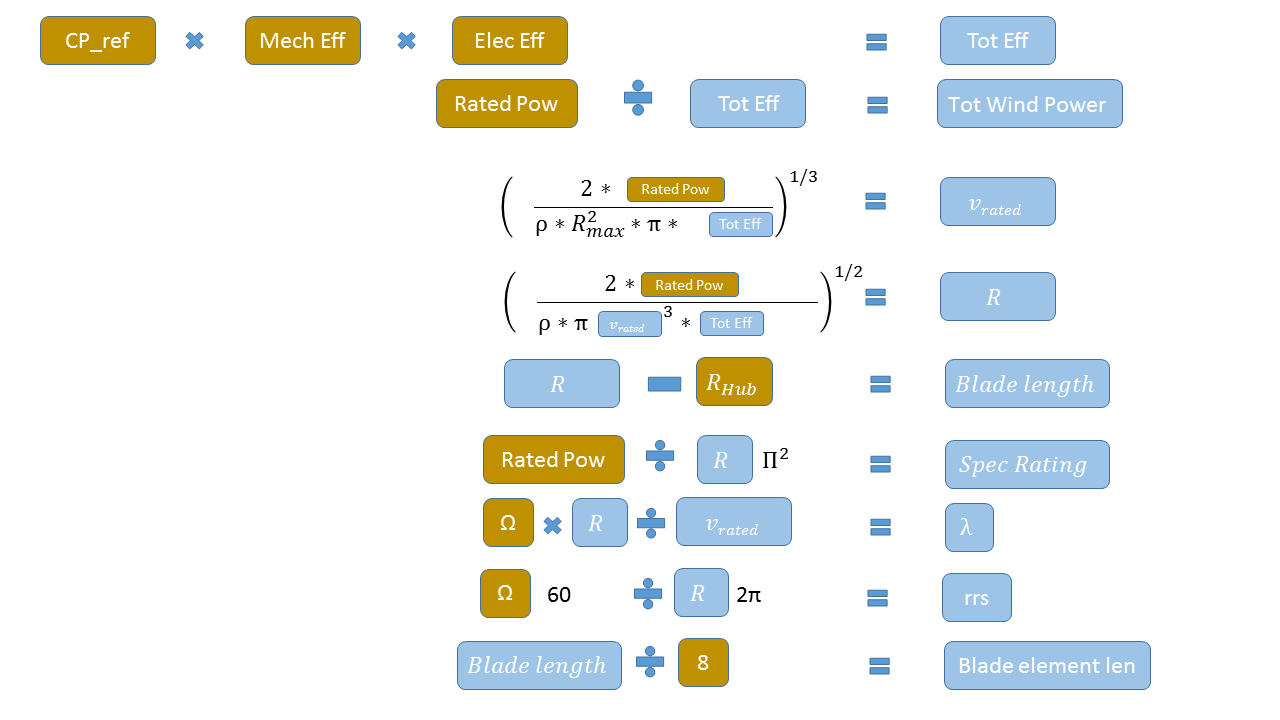
\includegraphics[width=\linewidth]{figures/cip1_params.png}
\end{figure}
\end{frame}

\begin{frame}
\huge
Results
\begin{table}
\footnotesize
\centering
\begin{tabular}{ | l | l | l | }
\hline
	\textbf{Main parameters} & \textbf{Unit} & \textbf{Value} \\ \hline \hline
	Calculate total conversion efficiency & m & 0.4704 \\ \hline
	Total wind power that needs to be extracted & kW & 7439.258 \\ \hline
	Rated wind speed (rounded up) & m/s & 11 \\ \hline
	Rotor radius (rounded up) & m & 54 \\ \hline
	Blade length (without hub) & m & 52.75 \\ \hline
	Rotor area (rounded radius) & $m^2$ & 9160.884 \\ \hline
	Specific rating (design) & $W/m^2$ & 382.051 \\ \hline
	$\lambda D$ Design tip speed ratio & - & 7.454 \\ \hline
	Rotor rated speed & rpm & 14.5 \\ \hline
	Blade element length (8 elements, same length) & m & 6.593 \\ \hline
\end{tabular}
\end{table}
\end{frame}

\begin{frame}
\huge
Estimation of AEP
\begin{figure}[htbp]
	\begin{center}
		\begin{minipage}[t]{0.4\linewidth}
			\centering
			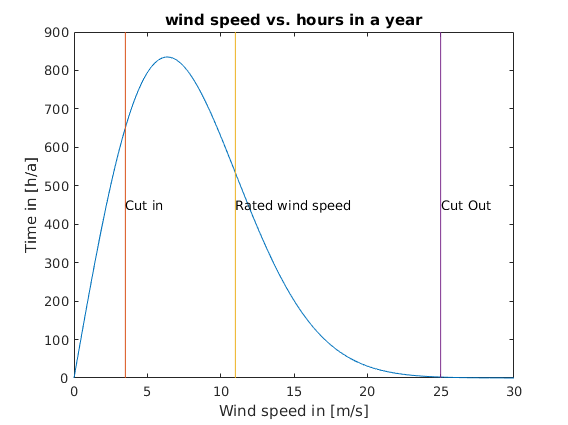
\includegraphics[width=\linewidth]{figures/ws_plot.png}
		\end{minipage}
		\begin{minipage}[t]{0.4\linewidth}
			\centering
			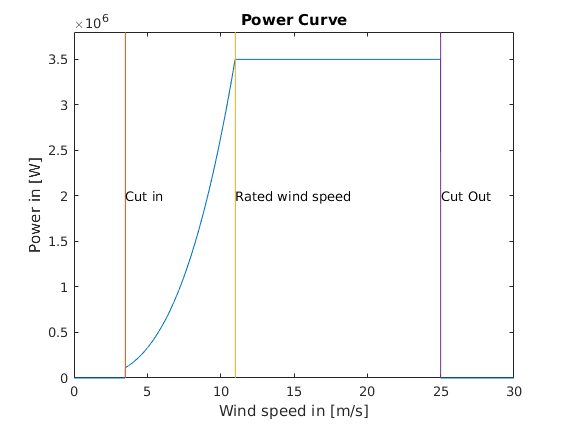
\includegraphics[width=\linewidth]{figures/power_curve.png}
		\end{minipage}
	\end{center}
\end{figure}
\footnotesize
\begin{equation*}
\text{AEP} = \sum_v n_v \cdot p_v
\end{equation*}
\scriptsize
with: \\
n = number of hours \\
p = power curve\\
v = wind speed\\

\end{frame}

\begin{frame}
\huge
Resulting Energy yield
\begin{figure}[htbp]
\centering
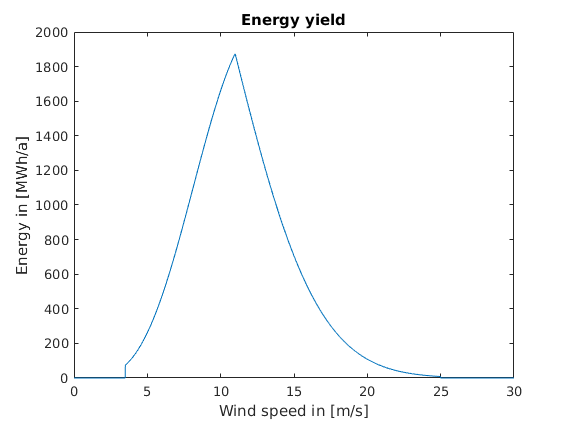
\includegraphics[width=0.7\linewidth]{figures/energy_yield.png}
\end{figure}
\footnotesize
\begin{equation*}
\text{AEP} = 13,49 GWh
\end{equation*}

\end{frame}

\begin{frame}
\huge
Lift-to-drag ratio
\begin{figure}[htbp]
	\begin{center}
		\begin{minipage}[t]{0.4\linewidth}
			\centering
			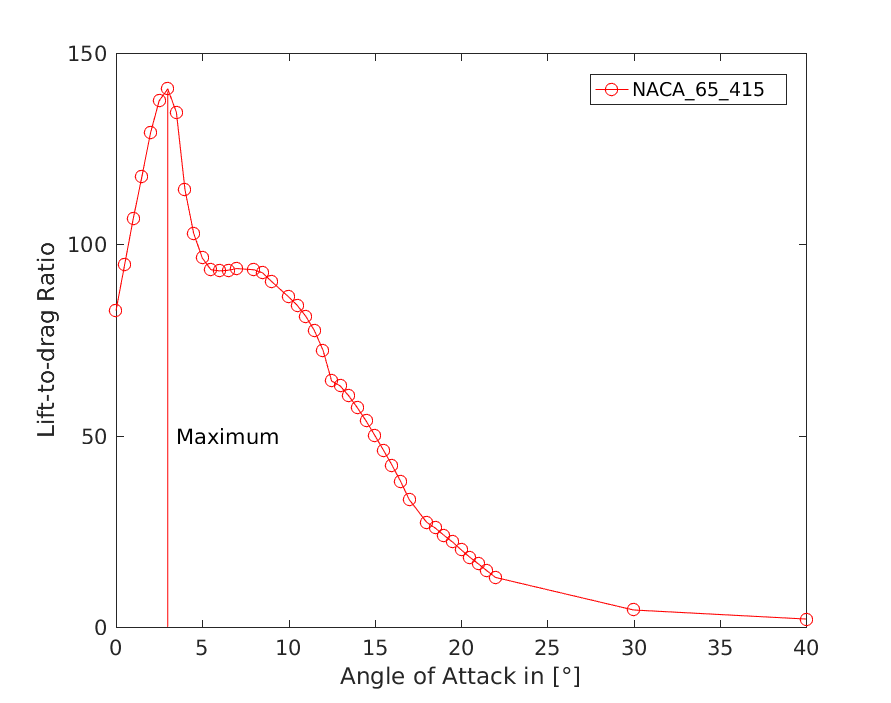
\includegraphics[width=\linewidth]{figures/lift_to_drag_ratio_415.png}
		\end{minipage}
		\begin{minipage}[t]{0.4\linewidth}
			\centering
			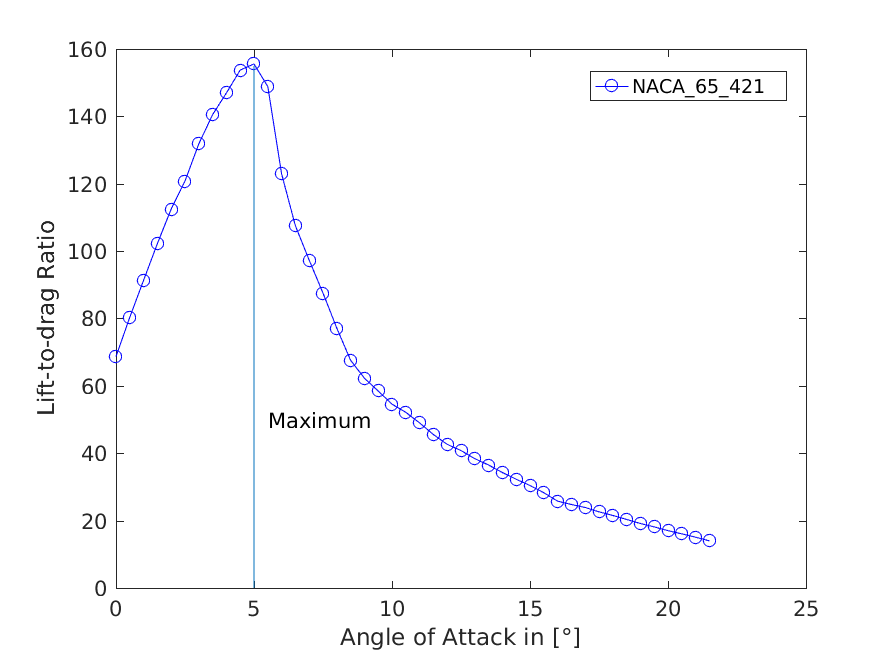
\includegraphics[width=\linewidth]{figures/lift_to_drag_ratio_421.png}
		\end{minipage}
	\end{center}
\end{figure}
\footnotesize
\begin{table}[H]
\begin{tabular}{l | r r r r}
NACA 65-415 & $\alpha$ &$c_l$ &$c_d$ & $c_m$\\
\hline
80\% method& 10 & 1.345 & 0.016 & 0.071\\
lift-to-drag method & 3.0 & 0.710 & 0.005 &  0.088\\
\hline
NACA 65-421 & $\alpha$ &$c_l$ &$c_d$ & $c_m$\\
\hline
80\% method& 11 & 1.255 & 0.026 & 0.055\\
lift-to-drag method & 5.0 & 0.952 & 0.006 &  0.092\\
\end{tabular}
\caption{Main aerodynamic parameters}
\end{table}
\end{frame}


\section{Rotor design, BEM}

\begin{frame}
\huge
Blade design
\Tiny
\begin{figure}[H]
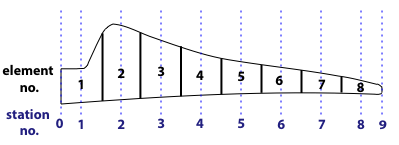
\includegraphics[width=0.6\linewidth]{../CIP_2/Figures/blade_elements.png}
\label{fig:blade_elemets}
\end{figure}
\begin{table}[H]
\begin{tabular}{c| l l l l l l l l l}
\hline
Station  & 	1&	2&	3	&4	&5	&6	&7	&8	&9\\
&Cylinder&65-421&65-421&65-421&65-421& 65-415& 65-415& 65-415&65-415\\
\hline
Blade&	3.297&	9.891&	16.484&	23.078&	29.672&	36.266&	42.859&	49.453&	52.750\\
\hline
Chord &	6,628	&5,426&	3,935	&3,014&	2,425&	1,887&	1,617&	1,413&	1,329\\
Twist &	27,590&	11,022&	3,813&	0,055&	-2,211&	-2,715&	-3,783&	-4,580&	-4,907\\
\hline
\end{tabular}
\label{final_blade_design_schmitz}
\end{table}
\end{frame}

\begin{frame}
\huge
BEM algorithm
\begin{figure}[H]
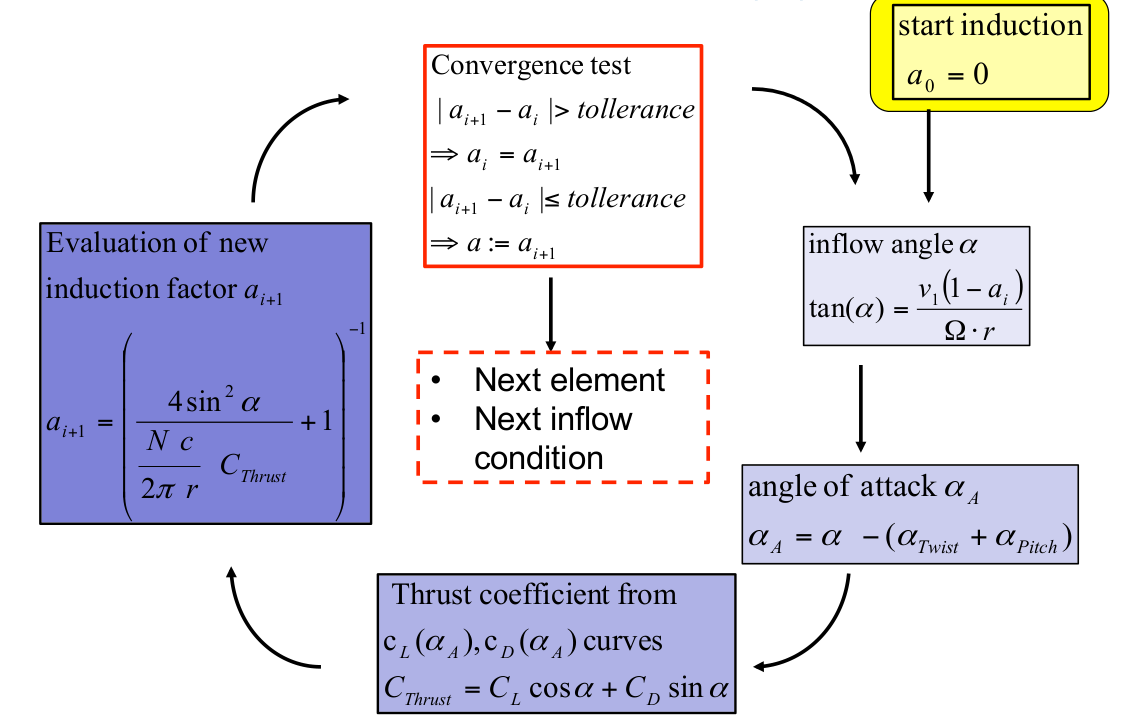
\includegraphics[width=0.8\linewidth]{figures/algo.png}
\label{fig:blade_elemets}
\end{figure}
\end{frame}

\begin{frame}
\huge
Prandtl tip losses
\Tiny
\begin{figure}[H]
\centering
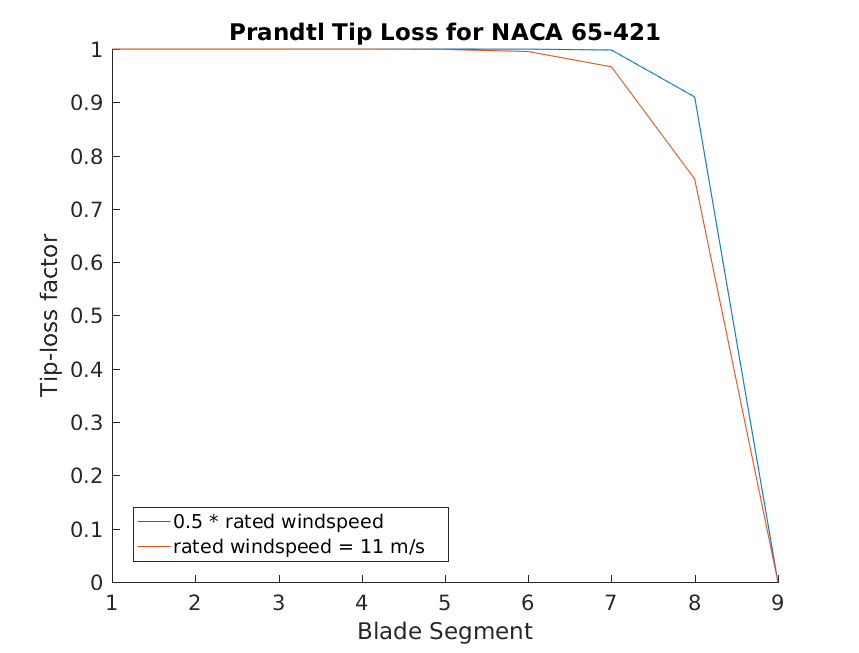
\includegraphics[width=0.8\linewidth]{../CIP_2/Figures/prandtl_tip_loss.png}
\end{figure}
\end{frame}

\begin{frame}
\huge
Pitching moment
\normalsize
\begin{equation*}
M= C_m \cdot A \cdot c \cdot \rho \cdot v^2 \cdot 0.5
\end{equation*}
\begin{figure}[H]
\centering
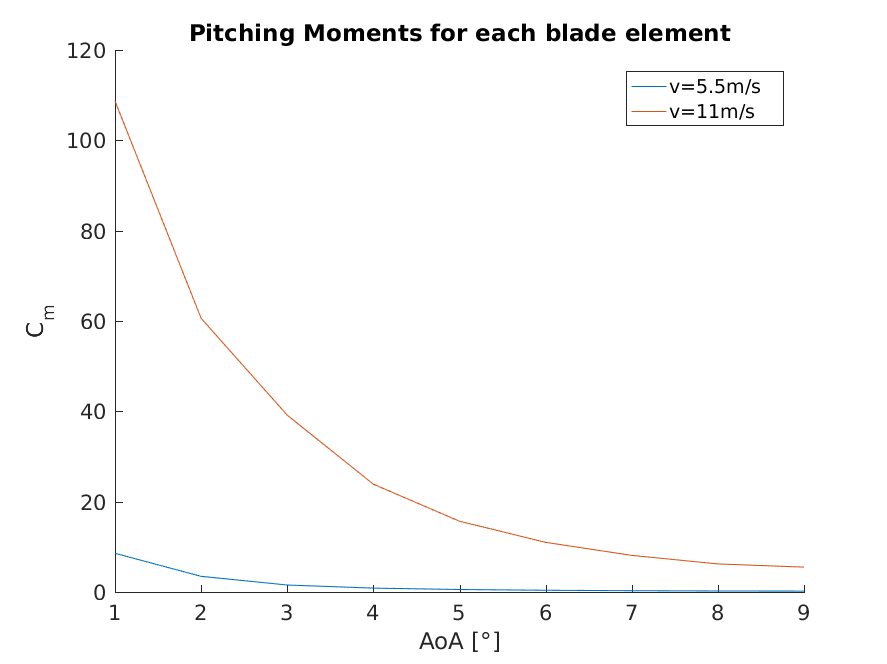
\includegraphics[width=0.5\linewidth]{../CIP_2/Figures/pitchingperbe.png}
\end{figure}
Result by summing up the sections along the blade
\begin{align*}
M(5.5m/s) &= 15.881 Nm\\
M(11m/s) &= 278.705 Nm
\end{align*}
\end{frame}

\section{Control and characteristic curves}
\begin{frame}
\Huge
WT\_Perf
\begin{figure}
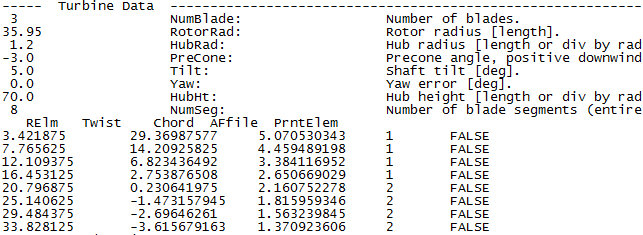
\includegraphics[width=0.6\linewidth]{figures/wt_perf.png}
\end{figure}

\begin{figure}[htbp]
        \begin{minipage}{0.4\linewidth}
            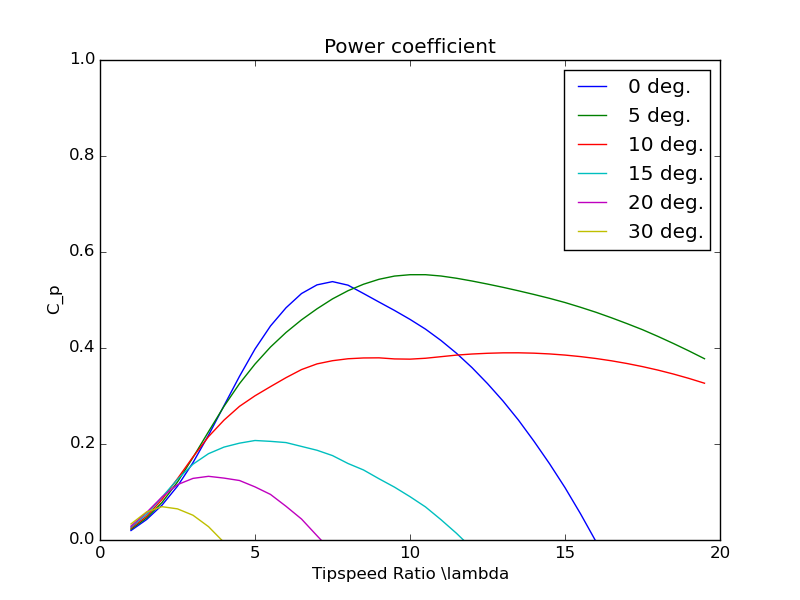
\includegraphics[width=\linewidth]{figures/cp.png}
        \end{minipage}
        \begin{minipage}{0.4\linewidth}
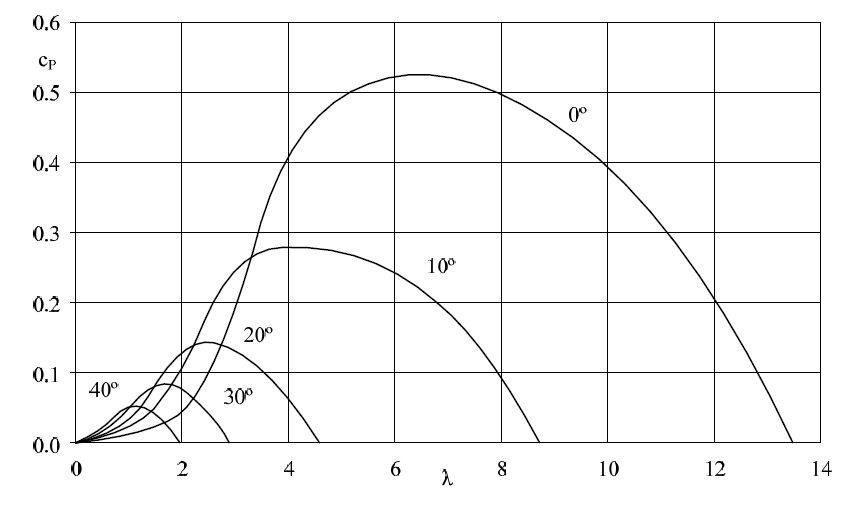
\includegraphics[width=\linewidth]{figures/power_coeff_literature.png}
        \end{minipage}
\end{figure}
\end{frame}
\begin{frame}

\begin{figure}[htbp]
        \begin{minipage}{0.4\linewidth}
            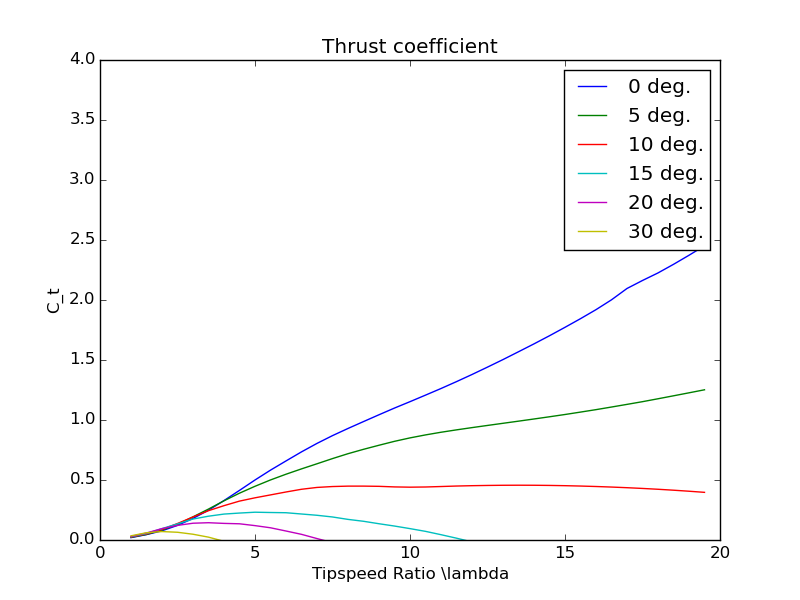
\includegraphics[width=\linewidth]{figures/thrust.png}
        \end{minipage}
        \begin{minipage}{0.4\linewidth}
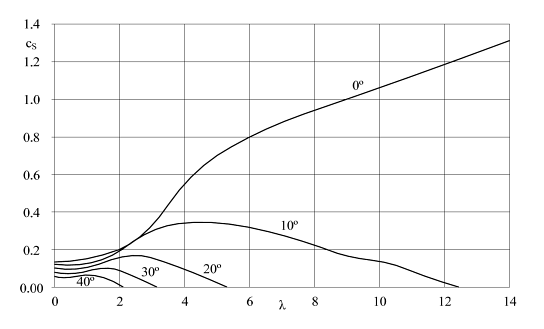
\includegraphics[width=\linewidth]{figures/thrust_coeff_literature.png}
        \end{minipage}
\end{figure}

\begin{figure}[htbp]
        \begin{minipage}{0.4\linewidth}
            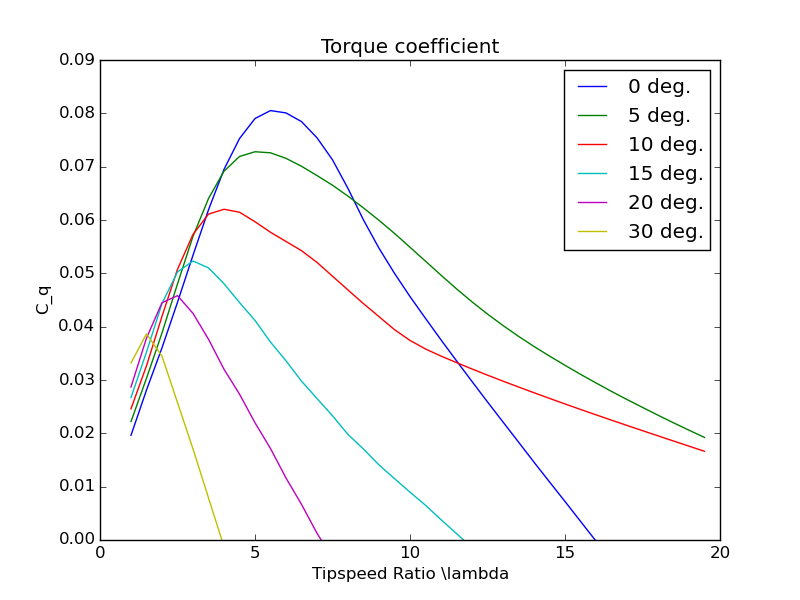
\includegraphics[width=\linewidth]{figures/torque.png}
        \end{minipage}
        \begin{minipage}{0.4\linewidth}
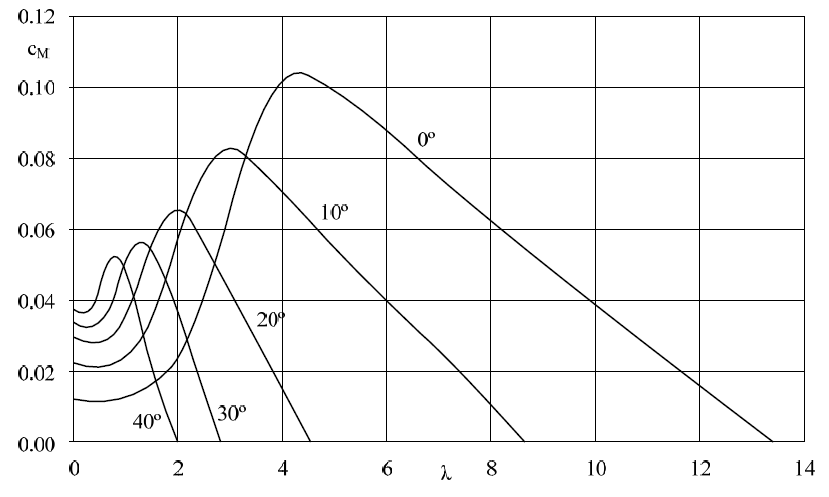
\includegraphics[width=\linewidth]{figures/torque_coeff_literature.png}
        \end{minipage}
\end{figure}
\end{frame}

\begin{frame}
How does the wind turbine operate below and above rated wind speed?\\
\begin{itemize}
\pause
\item[-] below rated wind speed it is still possible to achieve a high power coefficient $c_p$ for 9 m/s is 0.544
\pause
\item[-]if the wind speed is higher than the rated wind speed the power coefficient drops significantly
\pause
\item[-]Constant TSR leads to a high power coefficient
\end{itemize}
\end{frame} 


\section{Tower design, modal analysis}
\begin{frame}
\huge
Tower eigenfrequency\\[20pt]
\normalsize
Adding a $10 \%$ safety margin to the rotor rated speed which represents the maximum stationary rotor speed:
\begin{equation*}
	f_0 = \Omega_{rated} \cdot 1.1 = \frac{14.5}{60} Hz \cdot 1.1 = 0.2658 Hz
\end{equation*}
Design range: Classical soft-stiff design
\begin{figure}
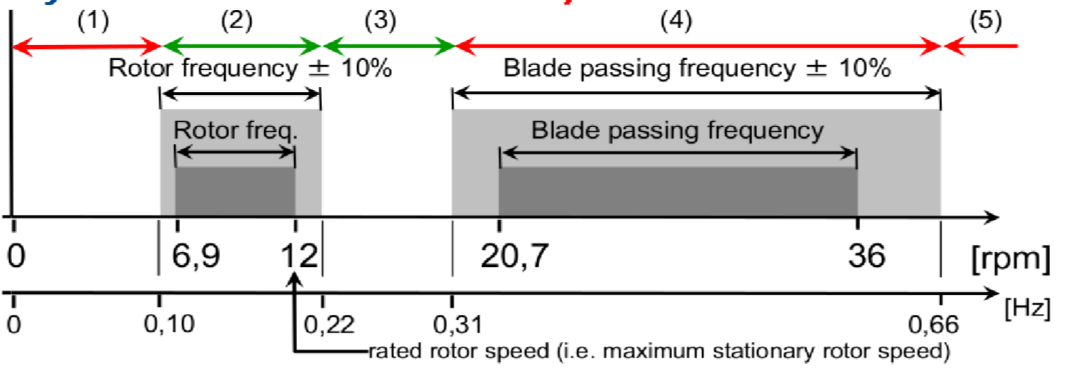
\includegraphics[width=0.8\linewidth]{figures/designranges.png}
\end{figure}
\end{frame}

\begin{frame}
\huge
Wall thickness \\[20pt]
\small
Can be obtained from the eigenfrequency and some other parameters
\begin{figure}[htbp]
        \begin{minipage}{0.3\linewidth}
        \scriptsize
			\begin{equation*}
			f_0 \cdot 2 \pi  = \sqrt{\frac{3 E \pi D^3 t}{l^3 8 (m_{top} + 0.25\rho \pi D t l)}}
			\end{equation*}
			With fsolve:  $t=0.0318m$ \\
			Costs: ca $195870 Euro$
        \end{minipage}
		\qquad
        \begin{minipage}{0.5\linewidth}
			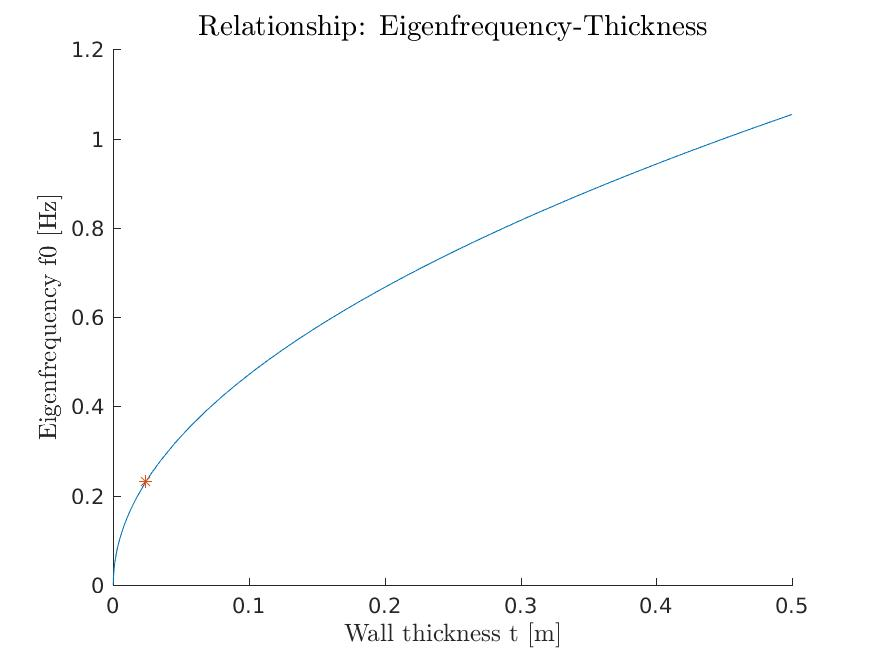
\includegraphics[width=\linewidth]{../CIP_4/figures/eigenfrequency.jpg}
        \end{minipage}
\end{figure}
\end{frame}

\begin{frame}
\huge 
Campbell diagram
\begin{figure}
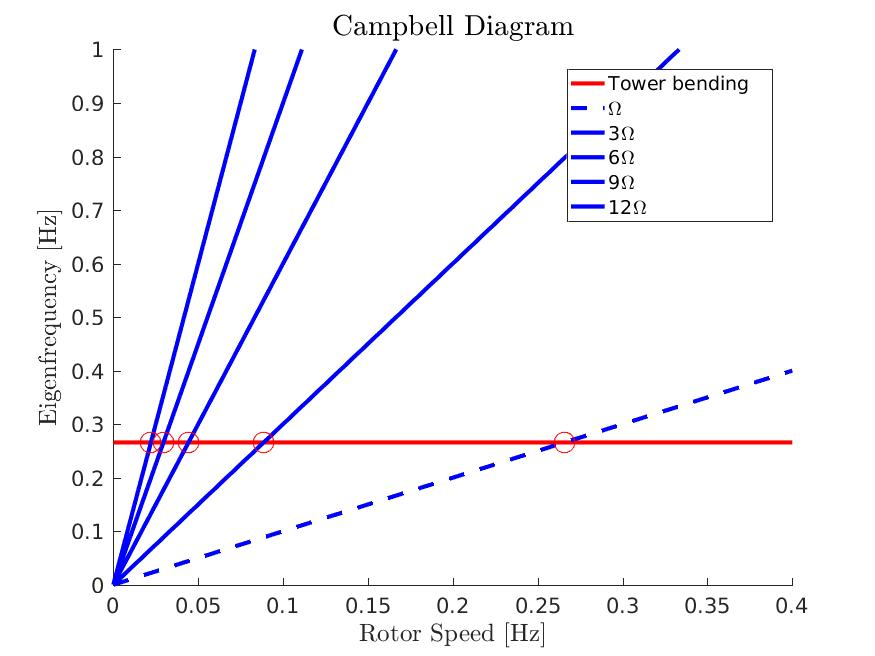
\includegraphics[width=0.8\linewidth]{../CIP_4/figures/campbell.jpg}
\end{figure}
\end{frame}

\section{External conditions}
\begin{frame}
\huge 
Software during the design process
\begin{figure}
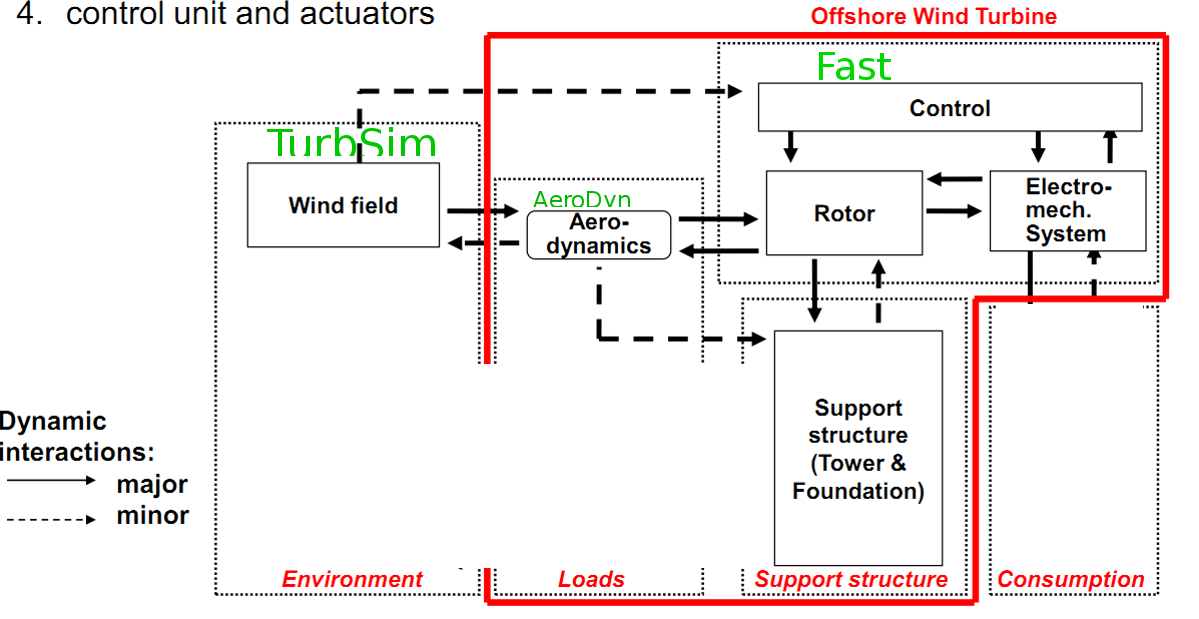
\includegraphics[width=0.8\linewidth]{figures/wind_turbine_overview.png}
\end{figure}
\end{frame}

\begin{frame}
\huge
Turbulence intensity \\[20pt]
\normalsize
Free stream (NTM)
\begin{align*}
 \sigma &= I_{ref}*(0.75*v_{hub}+5.6m/s) \\
     I &= \sigma/v_{hub}
\end{align*}
\begin{table}[H]
\centering
\begin{tabular}{| c | c | c | c | c |}
\hline
\textbf{v} & $5m/s$ & $10m/s$ & $15m/s$ & $25m/s$ \\
\hline
\textbf{I} & $0.2618$ & $0.1834$ & $0.1573$ & $0.1364$	\\
\hline
\textbf{Operational condition} & partial & partial & full & full	\\
\hline
\end{tabular}
\end{table}
\end{frame}

\begin{frame}
\normalsize
Wakes (Frandsen model)
\begin{align*}
 \sigma_T &= \sqrt{\frac{0.9 v_{hub}^2}{1.5+0.3 d_i \sqrt{V_{hub}/c}}+\sigma} \\
     I &= {((1-Np_w)\sigma^m+p_w*\sum_{i=1}^{N}\sigma_T^m(d_i))}^{1/m} \frac{1}{v_{hub}}
\end{align*}
\begin{table}[H]
\centering
\begin{tabular}{| c | c | c | c | c |}
\hline
\textbf{v} & $5m/s$ & $10m/s$ & $15m/s$ & $25m/s$ \\
\hline
$\mathbf{4 \cdot d}$ & $0.2667$ & $0.1867$ & $0.1594$ & $ 0.1370$	\\
\hline
$\mathbf{8 \cdot d}$ & $0.2621$ & $0.1827$ & $0.1562$ & $0.1349$	\\
\hline
\end{tabular}
\end{table}
\end{frame}

\begin{frame}
\huge
Comparison
\begin{figure}[H]
\centering
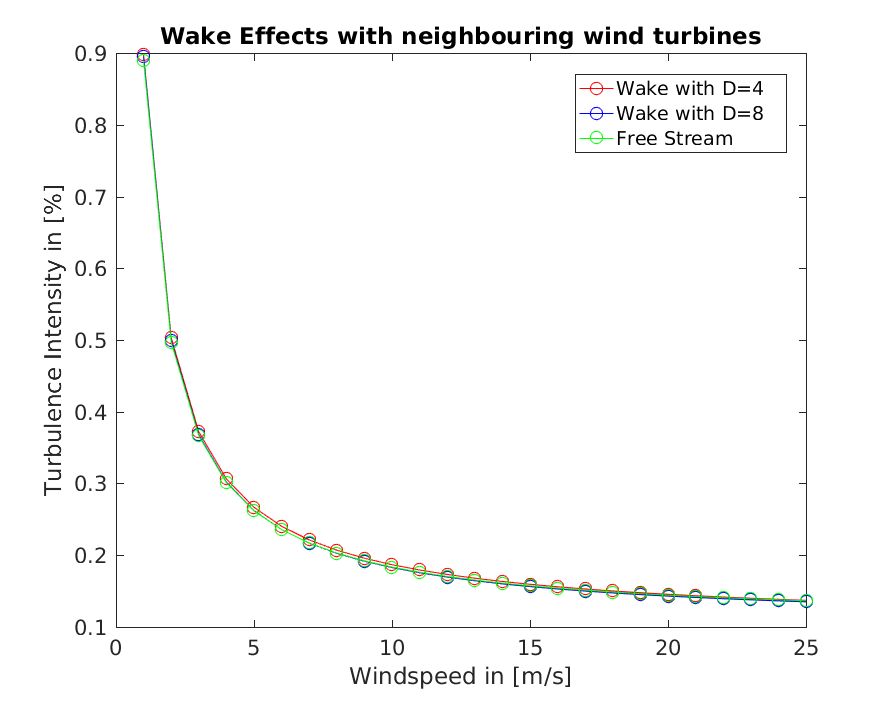
\includegraphics[width=0.9\linewidth]{../CIP_5/CIP_Tutorial_5_-_Windfield_and_wake_simulation/wake_effects_5.png}
\end{figure} 
\end{frame}

\begin{frame}

\begin{figure}[htb!]
\huge
Windfields\\[20pt]
\begin{minipage}{0.4\textwidth}
  \centering
  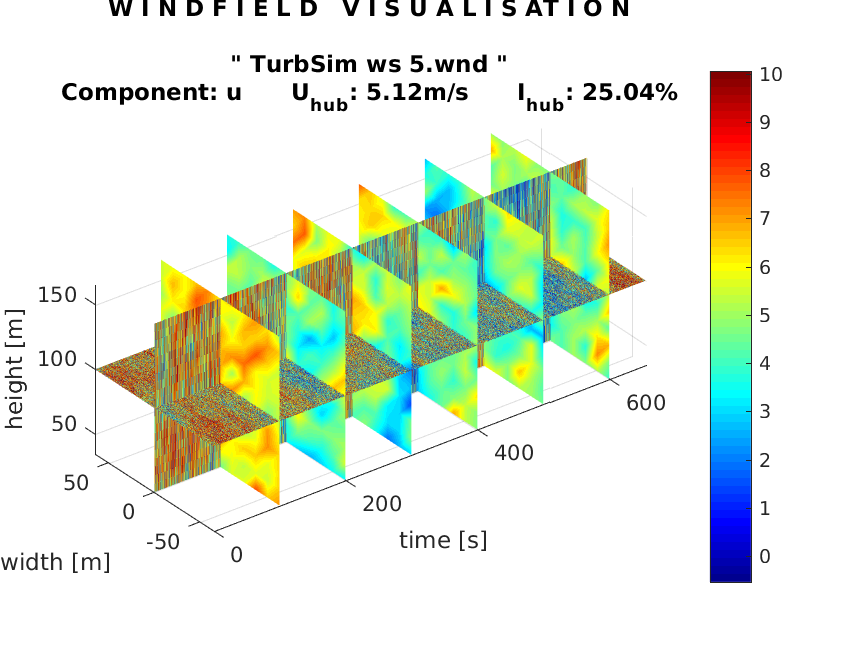
\includegraphics[width=1\linewidth]{../CIP_5/CIP_Tutorial_5_-_Windfield_and_wake_simulation/TurbSim/wind_5ms.png}
\end{minipage}
\begin{minipage}{0.4\textwidth}
  \centering
  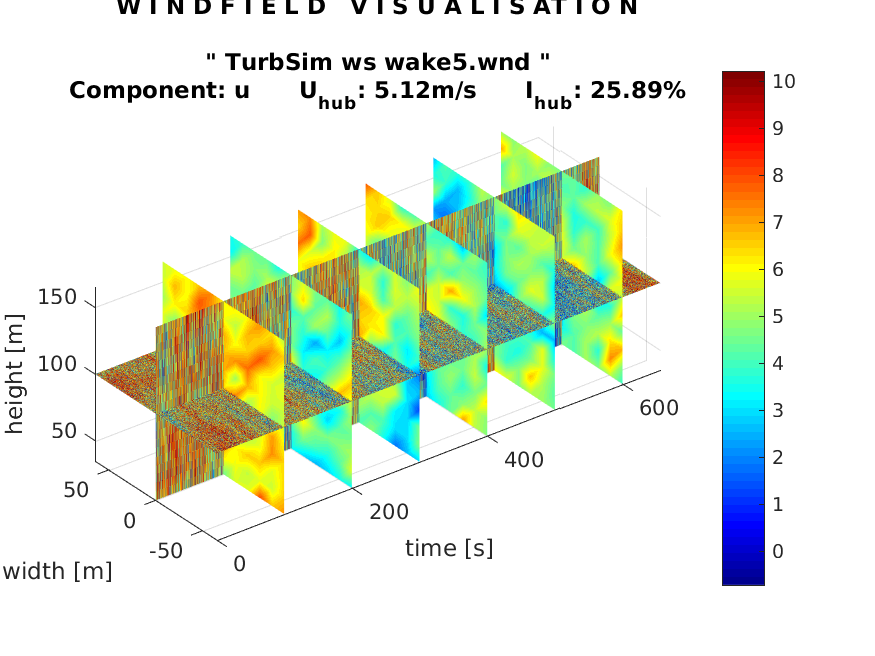
\includegraphics[width=1\linewidth]{../CIP_5/CIP_Tutorial_5_-_Windfield_and_wake_simulation/TurbSim/wind_wake_4_5ms.png}
\end{minipage}
\end{figure}
\end{frame}

\section{Fatigue load analysis}

\begin{frame}
\huge
Bending moments

\begin{figure}[H]
  \centering
\begin{minipage}{0.38\textwidth}
  \centering
  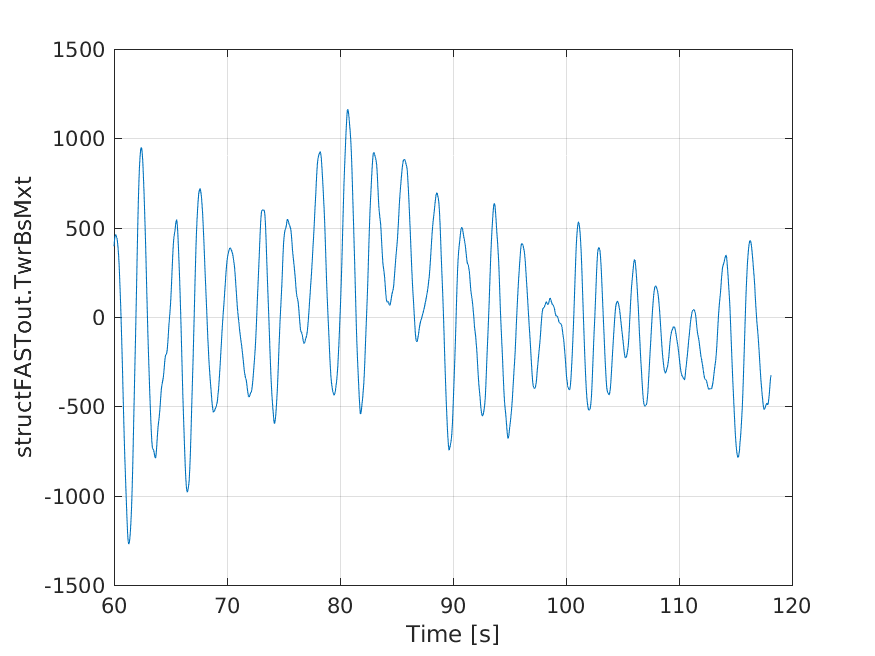
\includegraphics[width=1\linewidth]{../CIP_6/FAST/Plots_ws5/TwrBsMxt.png} \\
  \tiny
  Tower side-to-side bending moments
\end{minipage}
\begin{minipage}{0.38\textwidth}
  \centering
  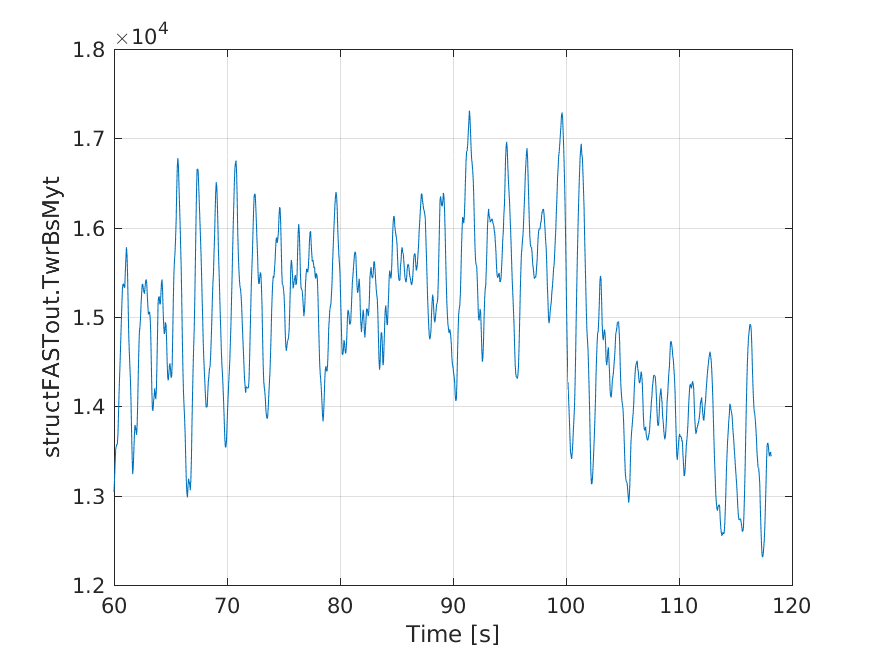
\includegraphics[width=1\linewidth]{../CIP_6/FAST/Plots_ws5/TwrBsMyt.png} \\
   \tiny
    Tower fore-aft bending moments
\end{minipage}
\begin{minipage}{0.38\textwidth}
  \centering
  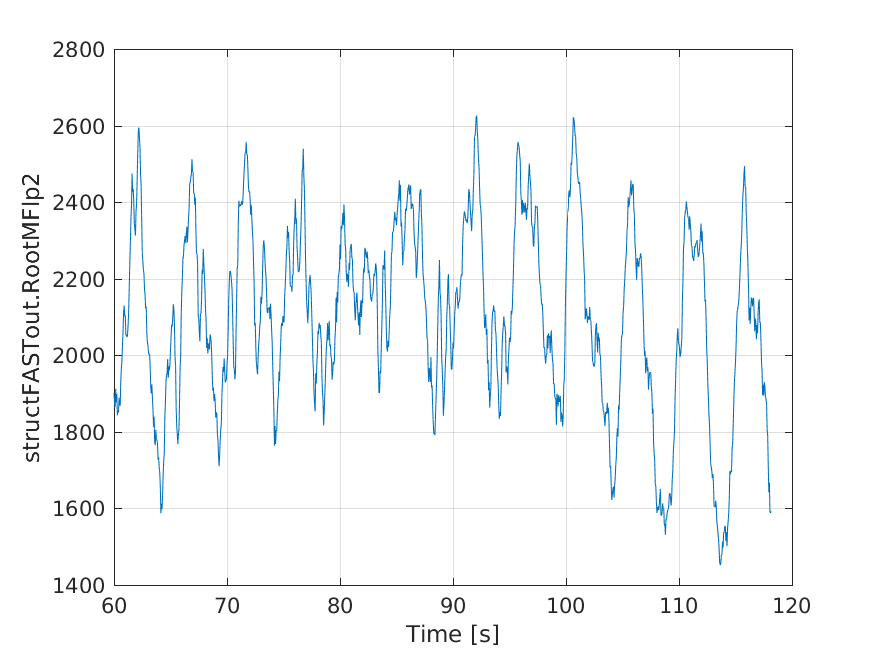
\includegraphics[width=1\linewidth]{../CIP_6/FAST/Plots_ws5/RootMFlp2.png} \\
     \tiny
      Blade flapwise bending moments
\end{minipage}
\begin{minipage}{0.38\textwidth}
  \centering
  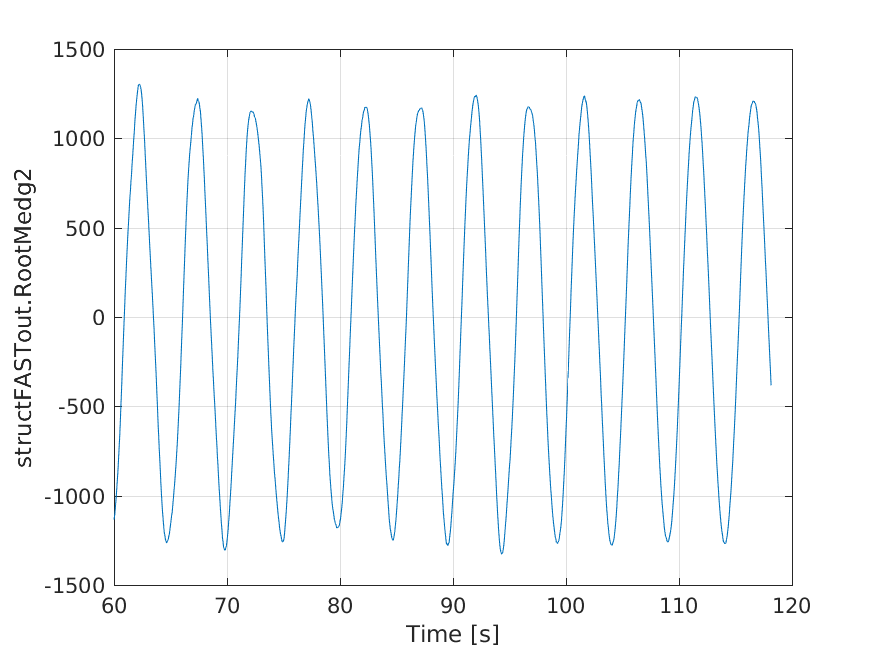
\includegraphics[width=1\linewidth]{../CIP_6/FAST/Plots_ws5/RootMedg2.png} \\
     \tiny
      Blade edgewise fore-aft bending moments
\end{minipage}
\end{figure}
\end{frame}

\begin{frame}
\Large
Comparison of DELs (free stream vs wake)
\begin{figure}[H]
  \centering
\begin{minipage}{0.40\textwidth}
  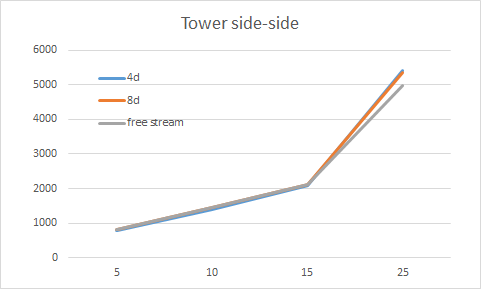
\includegraphics[width=1\linewidth]{figures/delsTwrSide.png}
\end{minipage}
\begin{minipage}{0.40\textwidth}
  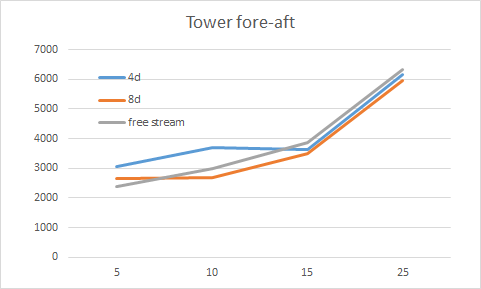
\includegraphics[width=1\linewidth]{figures/delsTwrFore.png}
\end{minipage}
\begin{minipage}{0.40\textwidth}
  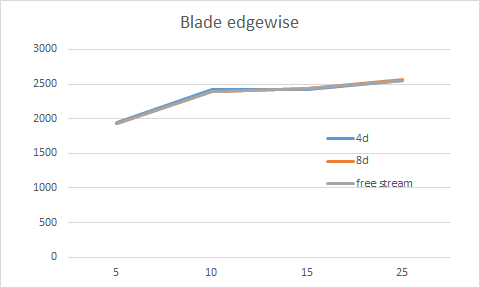
\includegraphics[width=1\linewidth]{figures/delsBldEdge.png}
\end{minipage}
\begin{minipage}{0.40\textwidth}
  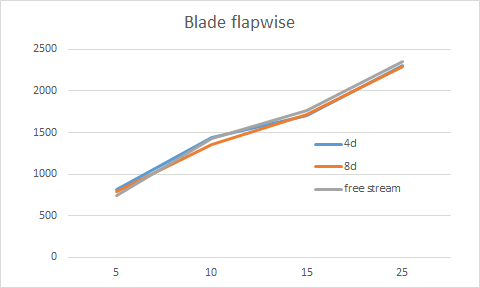
\includegraphics[width=1\linewidth]{figures/delsBldFlap.png}
\end{minipage}
\end{figure}
\end{frame}

\section{Extreme load analysis}
\begin{frame}
\huge
Loadcase 2.3
\begin{figure}[H]
  \centering
\begin{minipage}{0.40\textwidth}
  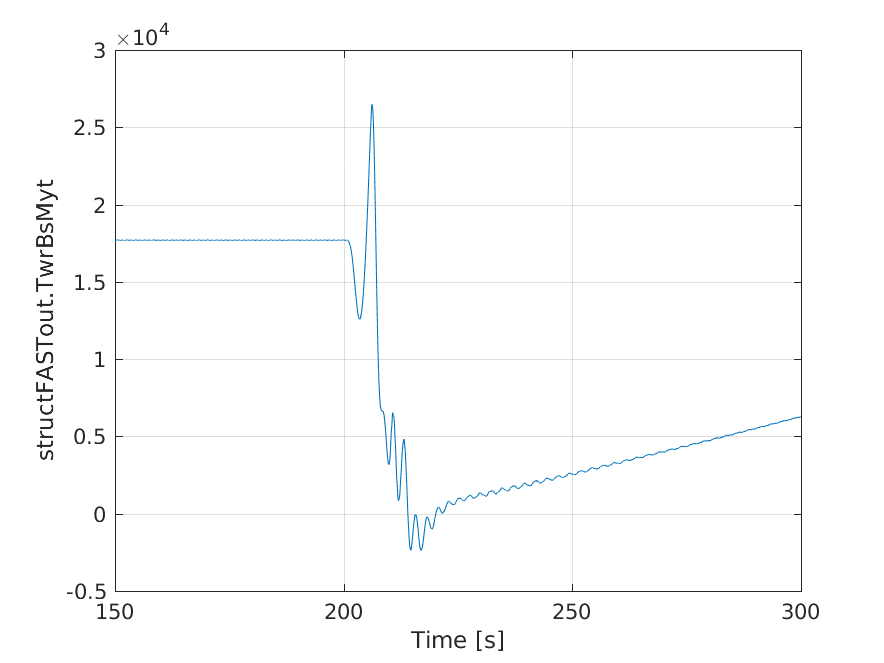
\includegraphics[width=1\linewidth]{../CIP_6/FASTextreme/EOG_50/TwrBsMyt.png} \\
  \centering
  \footnotesize
   Tower fore-aft for EOG\_50
\end{minipage}
\begin{minipage}{0.40\textwidth}
  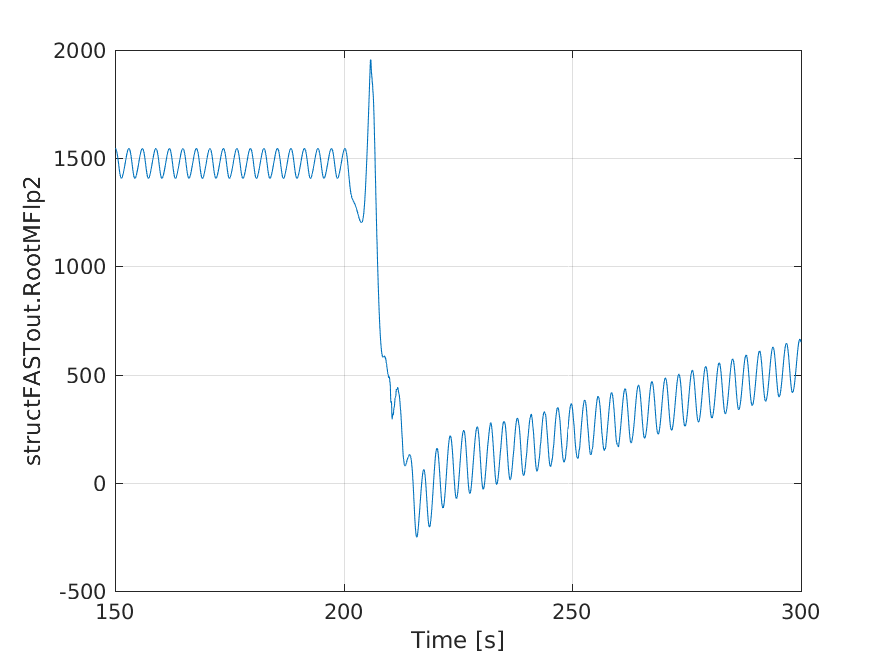
\includegraphics[width=1\linewidth]{../CIP_6/FASTextreme/EOG_50/RootMFlp2.png} \\
    \centering
      \footnotesize
   Blade flapwise for EOG\_50
\end{minipage}
\begin{minipage}{0.40\textwidth}
  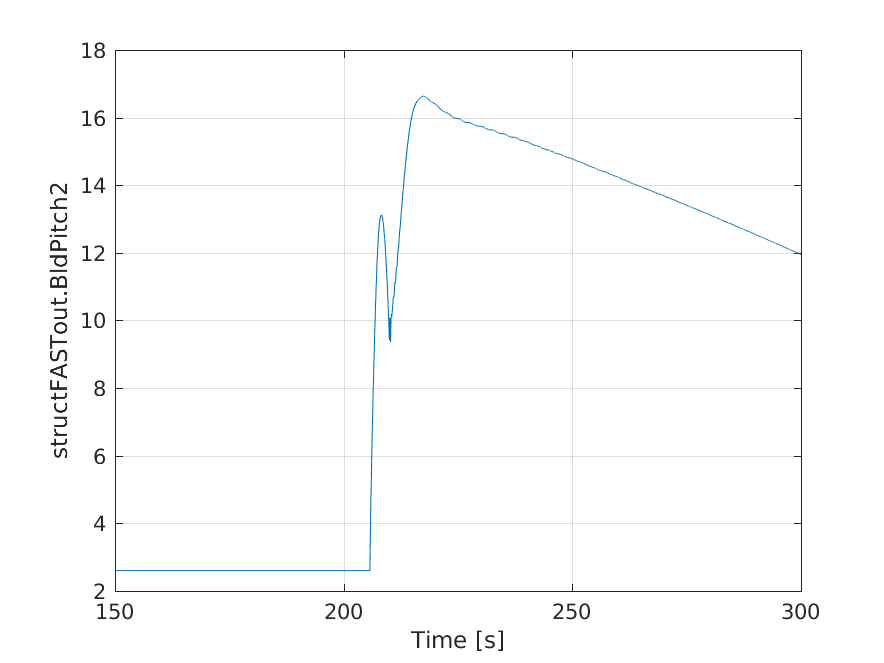
\includegraphics[width=1\linewidth]{../CIP_6/FASTextreme/EOG_50/BldPitch2.png} \\
    \centering
      \footnotesize
\end{minipage}
\end{figure}
\end{frame}

\begin{frame}
\huge
Loadcase 1.5
\begin{figure}[H]
  \centering
\begin{minipage}{0.40\textwidth}
  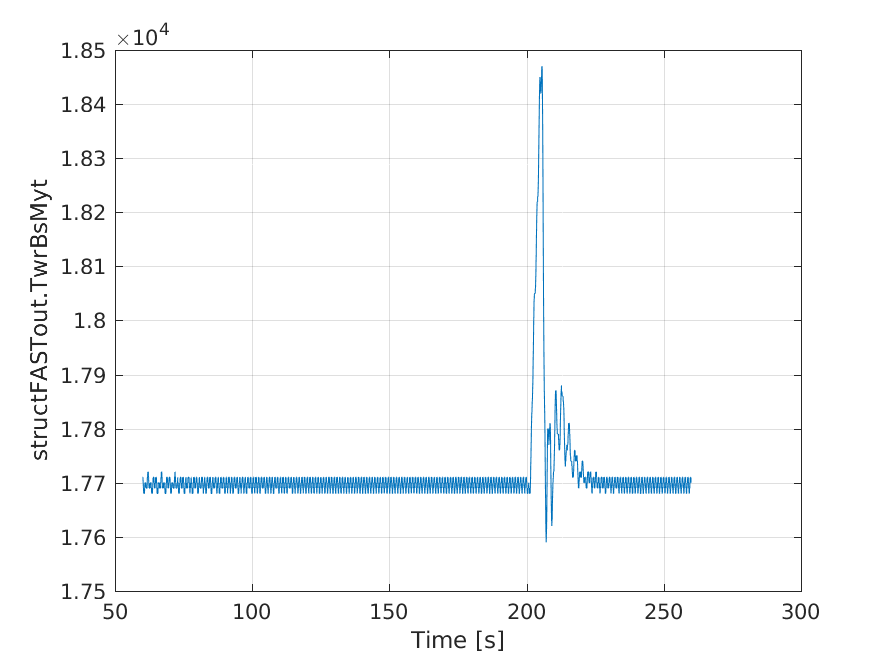
\includegraphics[width=1\linewidth]{../CIP_6/FASTextreme/EWSVR/TwrBsMyt.png}\\
      \centering
        \footnotesize
    Tower fore-aft for EWS
\end{minipage}
\begin{minipage}{0.40\textwidth}
  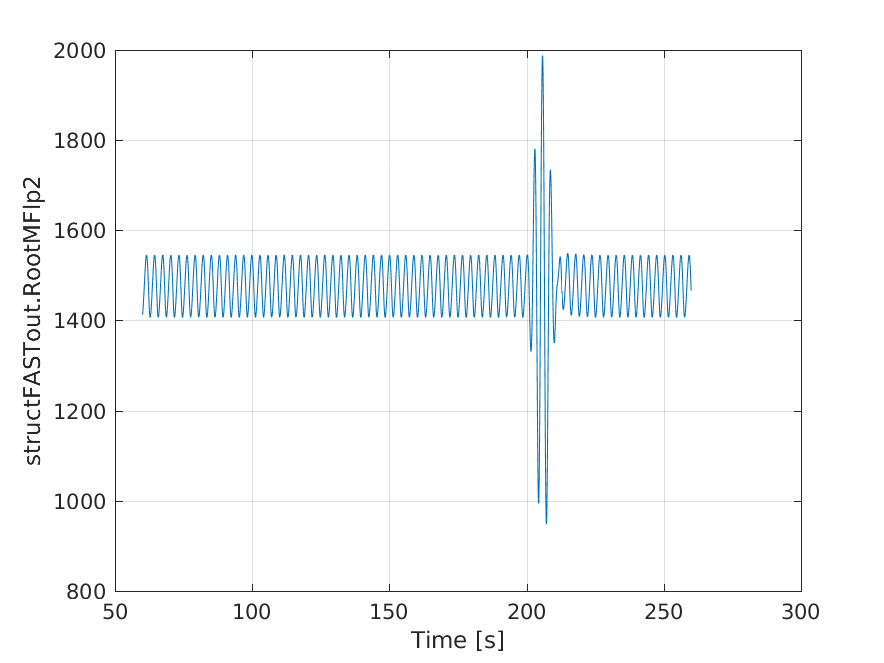
\includegraphics[width=1\linewidth]{../CIP_6/FASTextreme/EWSVR/RootMFlp2.png}\\
      \centering
        \footnotesize
    Blade flapwise for EWS
\end{minipage}
\end{figure}
\end{frame}

\begin{frame}
\Large
Modified brakes and failure timing 2.3
\begin{figure}[H]
  \centering
\begin{minipage}{0.38\textwidth}
          \centering
            \footnotesize
    Tower fore-aft
  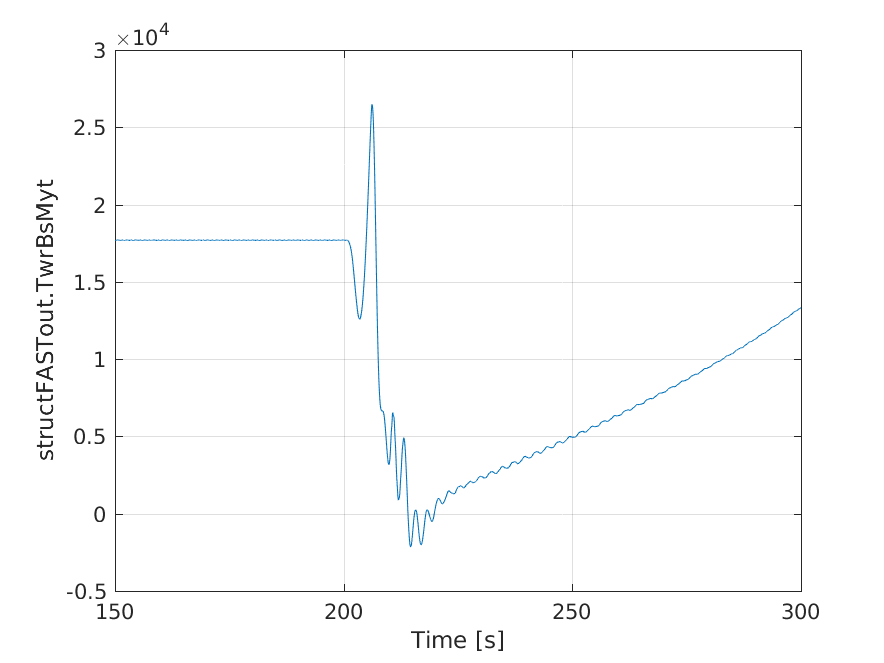
\includegraphics[width=1\linewidth]{../CIP_6/FASTextreme/EOG_50_brake/TwrBsMyt.png} \\
\end{minipage}
\begin{minipage}{0.38\textwidth}
          \centering
            \footnotesize
    Blade flapwise
  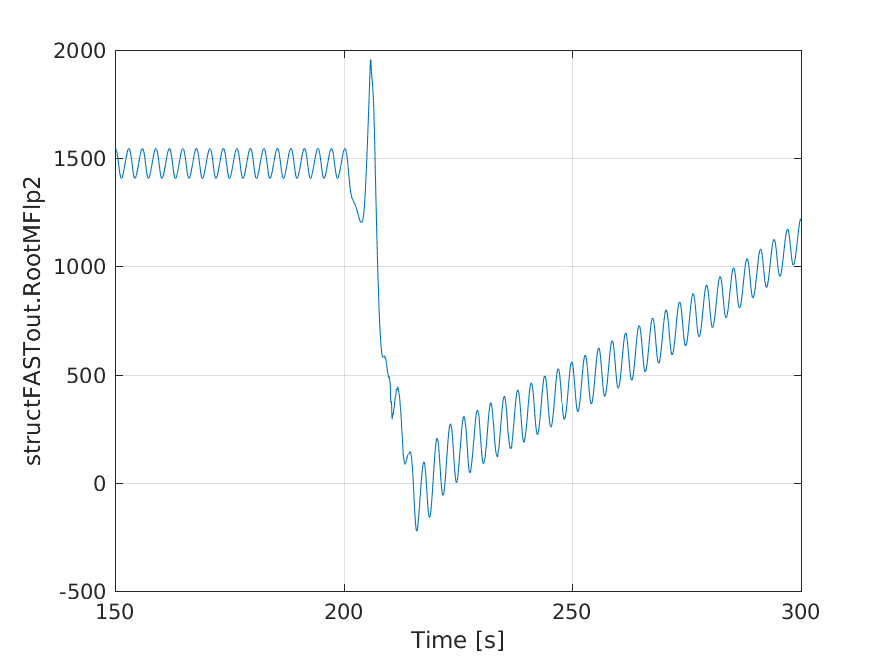
\includegraphics[width=1\linewidth]{../CIP_6/FASTextreme/EOG_50_brake/RootMFlp2.png}\\
\end{minipage}
\begin{minipage}{0.38\textwidth}
  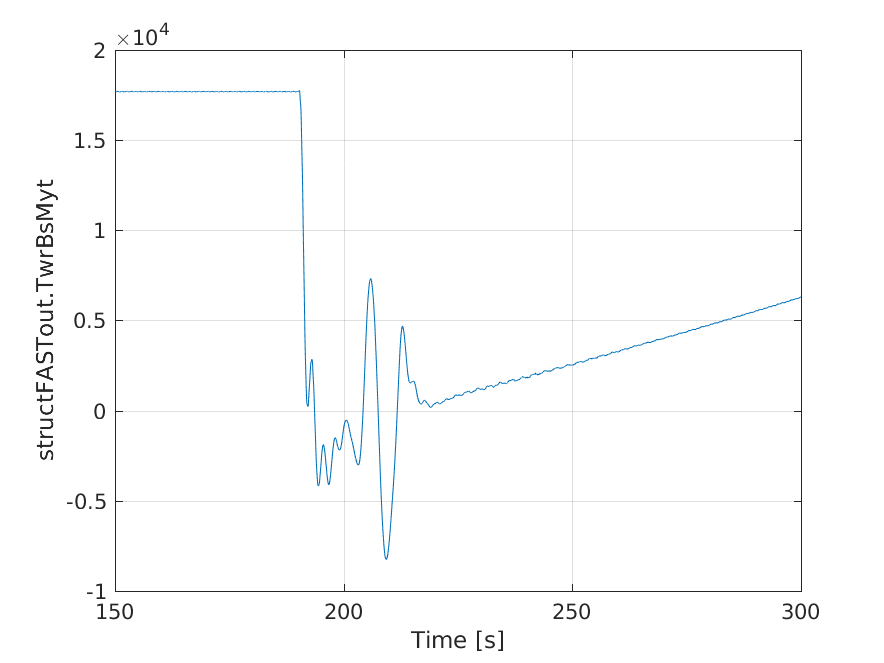
\includegraphics[width=1\linewidth]{../CIP_6/FASTextreme/EOG_50_failtime/TwrBsMyt.png} \\
\end{minipage}
\begin{minipage}{0.38\textwidth}
  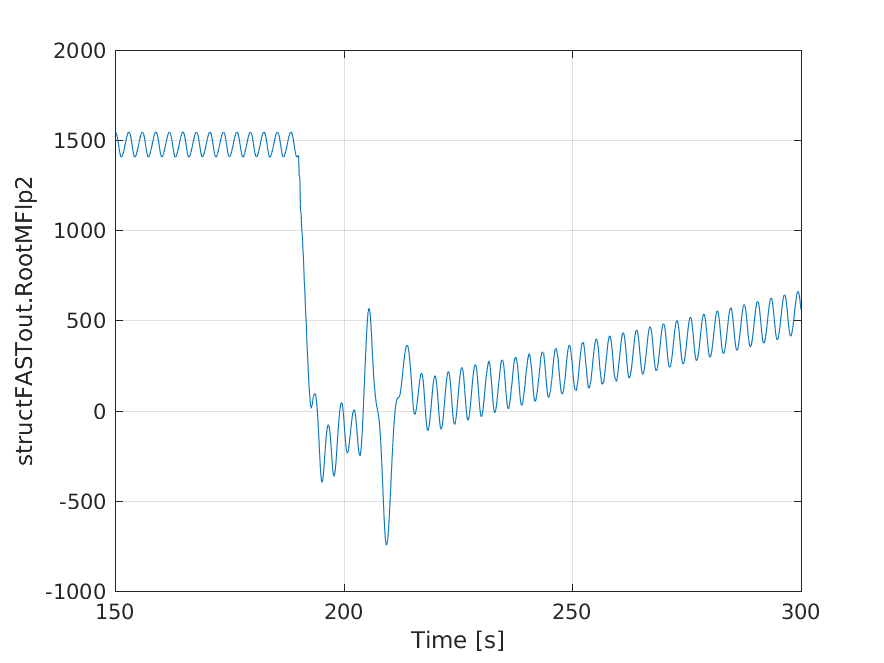
\includegraphics[width=1\linewidth]{../CIP_6/FASTextreme/EOG_50_failtime/RootMFlp2.png} \\
\end{minipage}
\end{figure}

\end{frame}


\begin{frame}[fragile]
\vspace{100 pt}
\Huge
\begin{center}
Thanks!
\end{center}
\end{frame}
%%%%%%%%%%%% End of content %%%%%%%%%%%%


\end{document}